\documentclass[a4paper,11pt]{exam}
    \usepackage{hyperref}
    \ifx\pdftexversion\undefined
       \usepackage{epsfig}
    \else
       \usepackage[pdftex]{graphics}
    \fi
    \usepackage{epsfig}
    \usepackage{verbatim}
\begin{document}
    \extraheadheight{.5in}
    \firstpageheader{\large\sf CS2105}%
    {\large\sf National University of Singapore\\ School of Computing \\
    \LARGE\sf Assignment 2}%
    {\large\sf Semester 2 13/14}
    \firstpageheadrule
    \pagestyle{headandfoot}

    \section*{Deadline}

    30 March, 2014 (Sunday), 11:59pm.

    \section*{Objective}

    In this assignment, you will implement a reliable transfer protocol on top of a unreliable channel that can drop packets or corrupt packets randomly (but always deliver packets in order).

    \section*{Pre-requisite}

You are expected to be familiar with the alternating bit protocol (rdt 3.0).

The assignment will be done under a controlled UNIX environment. Familiarity with UNIX environment (how to copy/move/delete/edit files, how to compile and run programs, etc.) is assumed.

\section*{Administrative Matters}

This is an \textit{individual} assignment.

An account has been setup for you on host cs2105-z.comp.nus.edu.sg. To access your account, ssh to the host and login using your SoC UNIX username and password \textit{from a SoC host or through SoC VPN}.

If you have any questions or encounter any problems with the steps discussed in the assignment, please contact the teaching staff through CS2105's blog.

\section*{Introduction}

For this assignment, you are given the code for a receiver and sender for three network layers: application, reliable transport (RDT), and unreliable transport (UDT).

The \texttt{UDTSender} and \texttt{UDTReceiver} classes simulate a networking layer that delivers packets unreliably.  A packet can get loss or get corrupted randomly.  However, for simplicity, you can assume that this layer delivers packets in order.

The \texttt{FileSender} and \texttt{FileReceiver} classes implement a file transfer application for this assignment.  \texttt{FileReceiver} basically waits for a connection, receives a file, and saves the file onto the disk with a given name.  To run \texttt{FileReceiver}, use
\begin{verbatim}
  java FileReceiver <port> <filename>
\end{verbatim}
For example,
\begin{verbatim}
  java FileReceiver 9000 foo.zip
\end{verbatim}
listens on port 9000 for connection and dumps the bytes received into a file named \texttt{foo.zip}.

The \texttt{FileSender} program is basically a file uploader that connects to the \texttt{FileReceiver} and sends the data read from a given file to \texttt{FileReceiver}.  To run \texttt{FileSender}, 
\begin{verbatim}
  java FileSender <filename> <hostname> <port>
\end{verbatim}
For example, 
\begin{verbatim}
  java FileSender foo.zip sunfire.comp.nus.edu.sg 9000
\end{verbatim}
connects to a \texttt{FileReceiver} running on sunfire.comp.nus.edu.sg at port 9000 and uploads \texttt{foo.zip} to the server.

Obviously, \texttt{FileSender} and \texttt{FileReceiver} require data delivery to be reliable. This is where you come in.  

\section*{Your Tasks}

You are also provided with two classes, \texttt{RDTSender} and \texttt{RDTReceiver}, that interface between the application (\texttt{FileSender} and \texttt{FileReceiver}) and the unreliable data transport (\texttt{UDTSender} and \texttt{UDTReceiver}).  \texttt{RDTSender} and \texttt{RDTReceiver} should employ techniques from Lecture 3, including acknowledgement, retransmission, timeout, and sequence number, to make sure that data to be delivered from ``above'' is sent correctly to the other side.   You need not, however, implement windowing nor checksum.  You can assume that a corrupted packet can be magically detected through checking the \texttt{isCorrupted} flag of a packet.

So, your task in this assignment is to modify the given \texttt{RDTSender.java} and \texttt{RDTReceiver.java} such that \texttt{FileSender} and \texttt{FileReceiver} will work correctly -- the received file is exactly the same as the file uploaded.  

You should read the given set of source code carefully to understand the interaction between the different classes.  The code is documented and should be pretty self-explanatory.  There are only about 300 lines of code in total.

Figure 1 shows the overall relationship between the classes in this assignment.

\begin{figure}
	\begin{center}
	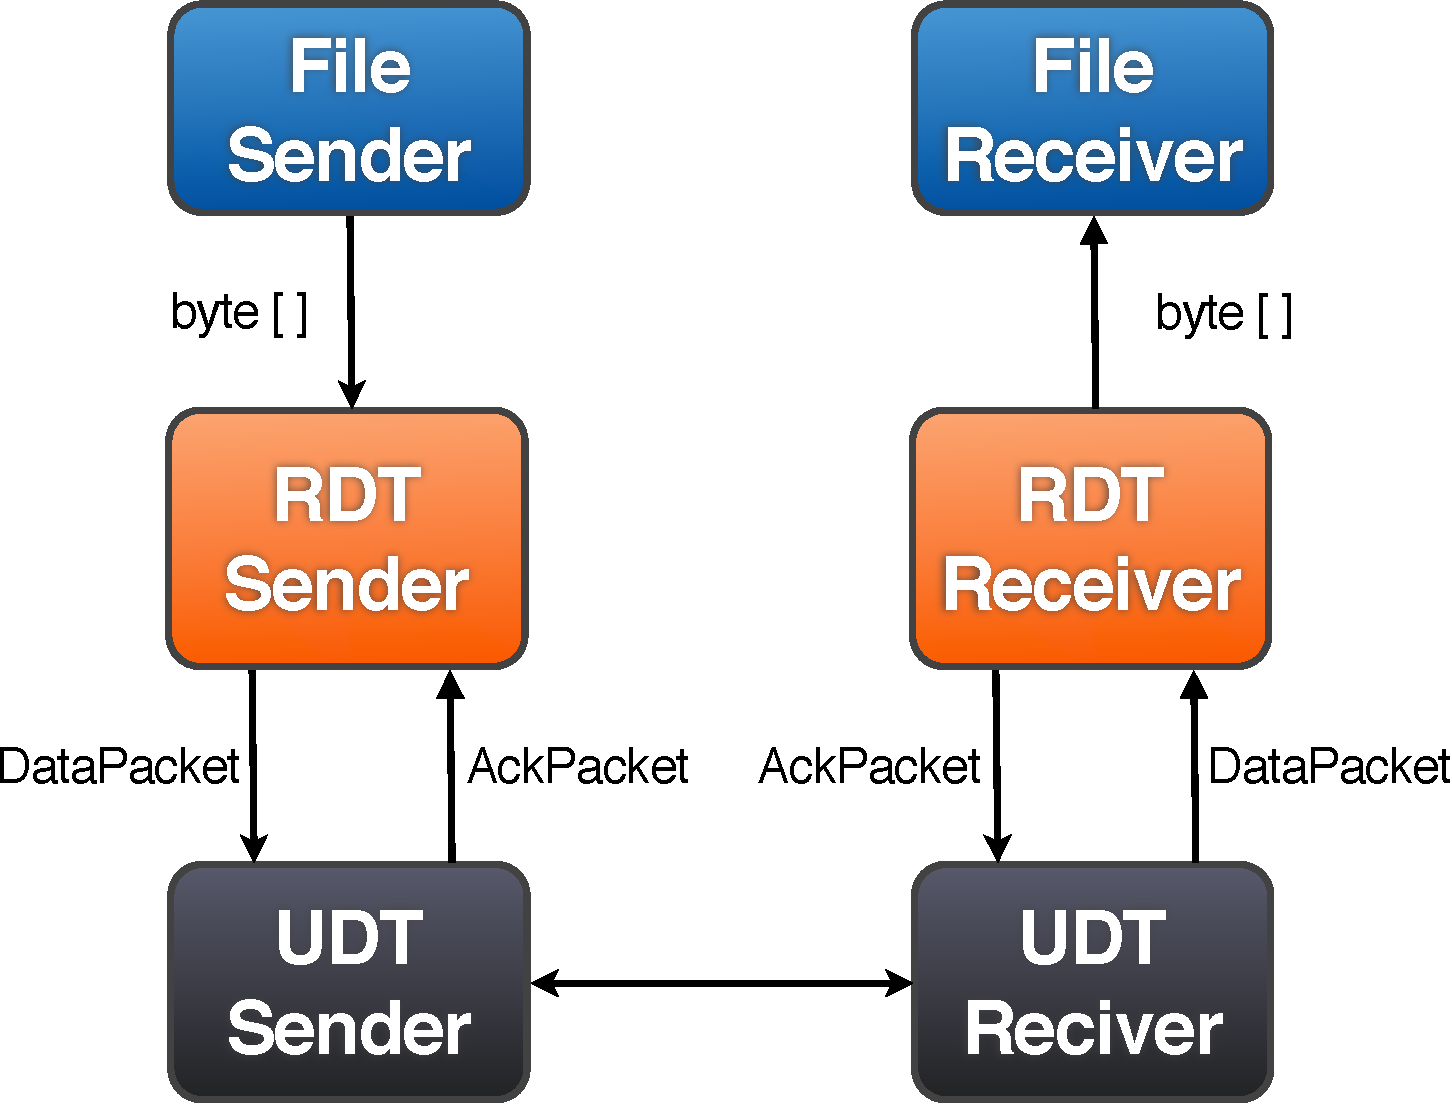
\includegraphics[scale=0.25]{flow-crop.pdf}
	\caption{Interaction between the Classes}
	\end{center}
\end{figure}

\section*{How to Do It in Java}

\subsection*{Timer}

You will need two java.util.* classes to implement timeout.  
The \texttt{Timer} class schedules a task to be executed periodically after a certain delay, while the \texttt{TimerTask} class implements the code that you want to execute periodically.  For example, to print a given number after 5 seconds, and subsequently every 5 seconds, you create the following task, 
\newpage

\begin{verbatim}
class NumberPrinter extends TimerTask {
  int x;
  NumberPrinter(int toPrint) {
    x = toPrint;
  } 
  public void run() {
    System.out.println(x);
  }
}
\end{verbatim}
and schedule the timer elsewhere like this.
\begin{verbatim}
  Timer timer = new Timer();
  timer.schedule(new NumberPrinter(10), 5000, 5000);
\end{verbatim}
When you want to stop printing,
\begin{verbatim}
  timer.cancel();
\end{verbatim}

You can read the Java document on these two classes for more details.

\subsection*{Timers and Timeout Value}

Your implementation should work for any retransmission timeout values.  You should at least test your code with a timeout value of less than or equal to 5ms (to test the case with premature timeout) and 100ms.

\subsection*{Sending and Receiving Packets}

(This operation has been done for you, so this section is for your information only)

To send and receive packets, the given code uses object serialization.  Two types of packets are defined, \texttt{DataPacket} and \texttt{AckPacket}.  They are implemented in \texttt{DataPacket.java} and \texttt{AckPacket.java} respectively.  Both classes implement the Java object serialization interface, which allows an object to be ``serialized'', i.e., to be converted into a byte stream that can be written somewhere (for instance, to disk, to a socket).  The byte stream can be read and transformed back into an object.

To send and receive data packets and ack packets, the given code wraps an object I/O stream around a socket, and calls \texttt{readObject()} and \texttt{writeObject()} to read and write \texttt{DataPacket} objects and \texttt{AckPacket} objects, effectively sending and receiving packet objects between the sender and the receiver.

\subsection*{Dropping and Corrupting Probability}

The UDT layer randomly corrupts or drops packets according to the probability \texttt{P\_DROP} and \texttt{P\_CORRUPT} respectively.  You can set these value to anything you want during testing.  If you have trouble getting the code to work, it might be useful to set one or more of these variables to 0 for debugging purposes.

\subsection*{Detecting Closed Connection}
One practical issue that needs to be dealt with for rdt 3.0 is the closing of the connection.  In this assignment, the sender sends a packet with no data (0 byte) to signal that there is no more packet.  The receiver closes the connection when it receives all the data correctly.  This action may lead to an \texttt{EOFException} being thrown at the sender.

You may handle this exception at the sender side by gracefully closing the connection (inside the \texttt{catch} block). You need not implement a TCP-like four-way handshake (FIN/ACK) to close the connection.

\section*{Verifying The Received File}
One way to check if the file received is the same as the file sent is to use cryptographic hash functions (Lecture 8).

On cs2105-z, the command \texttt{digest} can be used to compute a hash value for a file.  Different algorithms can be used, including MD5 and SHA-1, two popular MAC hashing function.  Here is what you can do:
\begin{enumerate}
\item Check the hash value of the file you want to send.  Suppose the file is called \texttt{foo.zip}:
\begin{verbatim}
bash$ digest -a md5 foo.zip
6e47011c85bf4532141b726105e11c0a
\end{verbatim}
You will see a hex string printed after running the command.  That is the hash of your file computing using the MD5 algorithm.

\item Repeat the command above for the received file and compared its hash to the hash computed at the sender.  They must be identical if the two files are identical.  The chances that the file is corrupted during transmission but still produce the same hash value is small, due to the property of cryptographic hash function.
\end{enumerate}

\section*{Your cs2105-z Account}

An account on the server, cs2105-z.comp.nus.edu.sg, has been setup for you. From within SoC (or through SoC-VPN), ssh to cs2105-z using your SoC UNIX id and password.

Copy the files prepared for you to your home directory, by executing:

\begin{verbatim}
cp -r ~sadm/a2 .
\end{verbatim}

Note that you must put your files inside the directory \texttt{a2} directly under your home directory. 

You will be responsible for the security of your own source code. Please be careful and set the correct permission for your files. They should not be readable by anyone else except the owner (chmod 600 *.java will ensure that).

Note that many of you will be running \texttt{FileReceiver} on the same host, and therefore must use a different port number. To prevent collision, you should avoid "nice" port numbers such as 8000 or 8080.

\section*{Submission and Grading}

There is no need to submit the program by email or IVLE workbin. We will collect your assignment from your home directory on cs2105-z.comp.nus.edu.sg when the deadline is over.

We will test your assignment automatically using a grading program. For this to work, you must not modify other java files (except \texttt{RDTSender} and \texttt{RDTReceiver}) in any signficant way (changing loss/corruption probability and adding printing debugging statement is OK).  If you suspect that there is a bug in these code, please contact us by posting on the blog.  

You MUST name your java program \texttt{RDTSender.java} and \texttt{RDTReceiver.java}.  We will only compile these two files when we grade. You MUST not implement additional classes in other *.java files.

\section*{Using Another Platform}

If you like to work on your assignment on other platforms (Windows, Mac) that you are more familiar with, you are free to do so. But when you submit your assignment, you should ensure that your program runs properly under cs2105-z.comp.nus.edu.sg and your java code is located under \$HOME/a2 on cs2105-z.comp.nus.edu.sg.

\section*{Plagiarism Warning}

You are free to discuss the assignment with your peers. But, ultimately, you should write your own code. We employ zero-tolerance policy against plagiarism. If you are caught copying from other student, or let others copy your code, you will receive zero for this assignment. Further disciplinary action may be taken by the school.

\section*{Grading}

\begin{itemize}
\item 3 marks: Correctly handle corrupted packets.
\item 3 marks: Correctly handle duplicate packets.
\item 4 marks: Correctly handle lost packets.
\end{itemize}

We will deduct one marks for every failure to following instructions (wrong directory name, wrong filename, etc.)

\vfill
\center\Huge{THE END}
\end{document}
